\documentclass[10pt,a4paper]{article}

\usepackage[latin1]{inputenc}
\usepackage{amsmath}
\usepackage{amsfonts}
\usepackage{amssymb}
\usepackage{graphicx}
\usepackage{listings}
\title{Assignment No :A2}
\date{}
\author{Roll No.4431}


\begin{document}
\maketitle
\section{Title:}
Concurrent Quick Sort

\section{Problem Definition}
Using Divide and Conquer Strategies design a a class for Concurrent Quick Sort using C++.

\section{Learning Objectives}
\begin{enumerate}
\item To understand the concept of quick sorting.
\item To understand applications of quick sort algorithm.
\item To be able to parallelize the algorithmic challenges.
\end{enumerate}

\section{Learning Outcomes}
\begin{enumerate}
\item Ability to analyze problems and find strategic places of interest where quick sort can be utilised.
\item Understanding of parallel/concurrent programming.
\end{enumerate}


\section{Related Mathematics}
Let S be the solution perspective of the given problem.
\\\\The set S is defined as:
\\\\$S=\lbrace\ s,e,X,Y,F,DD,NDD,S_{c},F_{c}|\varnothing_{s}\rbrace$
\\\\Where,
\\\\s= Start state,  Such that $Y=\lbrace \varnothing \rbrace$ 
\\\\e= End state 
\\\\X= Input Set.
\\\\$X=\lbrace$ seq(x) $\mid$ x $\in$ Natural numbers $\rbrace$
\\\\Y=Output set.
\\\\$Y=\lbrace Sorted Sequence \rbrace $
\\\\F= Set of functions used.
\\\\F=$\lbrace getElements(), partition(), quickSort(), print() \rbrace$
\\\\getElements()= function to take the input from the user.
\\\\partition()= function to partition the sequence.
\\\\quickSort()= recursive function implementing the quick sort algorithm.
\\\\print()= function to print the sorted sequence.
\\\\DD=Deterministic data.
\\DD=
\begin{enumerate}
\item sequence follows proper constraints.
\item sort element exists.
\item sequence terminates.
\end{enumerate}
NDD= Non-deterministic data.
\\NDD= $\cup$ - DD


\section{State Transition diagram}
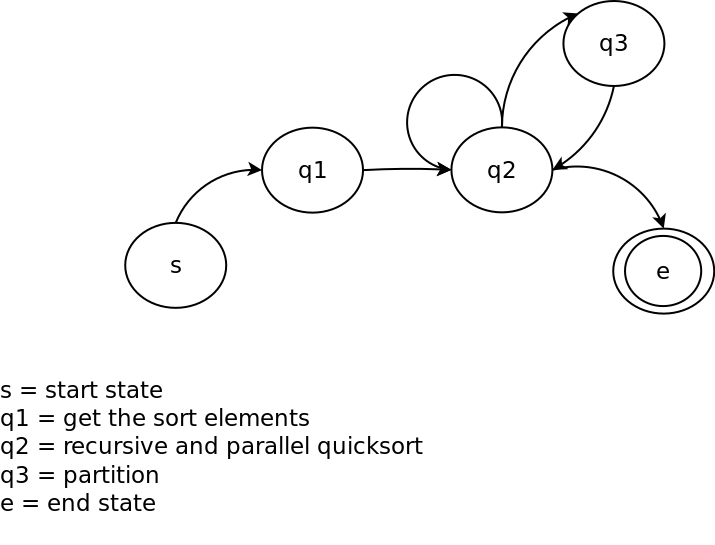
\includegraphics[scale=0.30]{stdg.png}

\section{Concepts related theory}
\subsection{Divide and Conquer : }
	\begin{itemize}
		\item Given a function to compute on an inputs the divide and conquer strategy suggest splitting the input into k distinct input sets ,such that 1<k<n yielding k sub problems.
		\item These sub problems must be solve and then method must be found to combine the sub solution into a solution of a whole.
		\item If the sub problems are relatively large then the divide and conquer strategy can be possibly reapplied.
		\item Often the sub problems are of the same type as the same original problem for which the reapplication of divide and conquer principle is naturally expressed by a recursive algorithm.
	\end{itemize}
	
	\subsection{Features of Quick Sort:}
	\begin{itemize}
		\item Similar to mergesort - divide-and-conquer recursive algorithm 
		\item One of the fastest sorting algorithms 
		\item Average running time O(NlogN) 
		\item Worst-case running time O(N2)
	\end{itemize}
	
	\subsection{Basic idea of Quick Sort:}
	\begin{enumerate}
		\item Pick one element in the array, which will be the pivot. 
		\item Make one pass through the array, called a partition step, re-arranging the entries so that: 
		\begin{itemize}
			\item the pivot is in its proper place. 
			\item entries smaller than the pivot are to the left of the pivot. 
			\item entries larger than the pivot are to its right. 
		\end{itemize}
		\item Recursively apply quicksort to the part of the array that is to the left of the pivot, and to the right part of the array. 
	\end{enumerate}
	
	\subsection{Algorithm : } We will dicuss the quicksort algorithm in detail,
	
	\begin{enumerate}
		\item Choosing the pivot \\ \textbf{ Choosing the pivot is an essential step.} Depending on the pivot the algorithm may run very fast, or in quadratic time.:
		\begin{enumerate}
			\item  Some fixed element: e.g. the first, the last, the one in the middle,this is a bad choice - the pivot may turn to be the smallest or the largest element, then one of the partitions will be empty.
			\item Randomly chosen (by random generator ) - still a bad choice. 
			\item The median of the array (if the array has N numbers, the median is the [N/2] largest number. This is difficult to compute - increases the complexity. 
			\item The median-of-three choice: take the first, the last and the middle element. Choose the median of these three elements. \\
			
			\textbf{Example:}\\
			8, 3, 25, 6, 10, 17, 1, 2, 18, 5 \\
			The first element is 8, the middle - 10, the last - 5. \\
			The median of [8, 10, 5] is 8
		\end{enumerate}
		
		\item Partitioning \\ \textbf{Partitioning is illustrated on the above example.}
		\begin{enumerate}
			\item The first action is to get the pivot out of the way - swap it with the last element \\
			5, 3, 25, 6, 10, 17, 1, 2, 18, 8\\
			\item  We want larger elements to go to the right and smaller elements to go to the left.Two "fingers" are used to scan the elements from left to right and from right to left:\\
			
			[5, 3, 25, 6, 10, 17, 1, 2, 18, 8]\\
			\^\qquad\qquad\qquad\qquad\qquad\qquad\^\\
			i \qquad\qquad\qquad\qquad\qquad\qquad j\\
			\begin{enumerate}
				\item  While i is to the left of j, we move i right, skipping all the elements less than the pivot. If an element is found greater then the pivot, i stops
				\item  While j is to the right of i, we move j left, skipping all the elements greater than the pivot. If an element is found less then the pivot, j stops
				\item  When both i and j have stopped, the elements are swapped.
				\item  When i and j have crossed, no swap is performed, scanning stops, and the element pointed to by i is swapped with the pivot .In the example the first swapping will be between 25 and 2, the second between 10 and 1.
			\end{enumerate}
			3. Restore the pivot.
			After restoring the pivot we obtain the following partitioning into three groups:\\
			$[5, 3, 2, 6, 1] [ 8 ] [10, 25, 18, 17]$
			
		\end{enumerate}
		
		\item Recursively quick sort the left and the right parts
	\end{enumerate}

\subsection{Code:}
	Here is the code, that implements the partitioning.\\
	left points to the first element in the array currently processed, right points to the last element. \\
	\lstset{language=C}          
	\begin{lstlisting}[frame=single] 
	if( left + 10 $<$= right)
	{
	int i = left, j = right - 1;
	for ( ; ; )
	{
	while (a[++i] $<$ pivot  ) {}  
	while (pivot  $<$ a[--j] ) {}   
	if (i $<$ j) swap (a[i],a[j]); 
	else  break;     
	}
	swap (a[I], a[right-1);  
	quicksort ( a, left, i-1);  
	quicksort (a, i+1, right);
	}
	else 
	insertionsort (a, left, right);
	\end{lstlisting}
	If the elements are less than 10, quicksort is not very efficient. 
	Instead insertion sort is used at the last phase of sorting.
	
	\subsection{Implementation notes:}
	Compare the two versions:
	\begin{enumerate}
		
		\item[A.] 
		while (a[++i] $<$ pivot) {}
		while (pivot $<$ a[--j]) {}
		
		if (i $<$ j) swap (a[i], a[j]);
		else break;
		\item[B.] \
		
		while (a[i] $<$ pivot) {i++;}
		while (pivot $<$ a[j] ) {j--;}
		
		if (i $<$ j) swap (a[i], a[j]);
		else break;
	\end{enumerate}
	If we have an array of equal elements, the second code will never increment i or decrement j, 
	and will do infinite swaps. i and j will never cross.
	
	
	\subsection{Concurrency in Quick sort:}
	\textbf{Concurrent Quicksort} \\
	\par	Simple concurrent implementation uses a collection of worker threads and a coordinator thread.The coordinator sends a message to an idle worker telling it to sort the array and waits to receive messages from the workers about the progress of the algorithm. \par
	A worker partitions a sub-array, and every time that worker gets ready to call the partition routine on a smaller array, it checks to see if there is an idle worker to assign the work to. If so, it sends a message to the worker to start working on the sub-problem; if not the current worker makes calls the partition routine itself.
	\par	After each partitioning, two recursive calls are (usually) made, so there are plenty of chances to start other workers.The diagram below shows two workers sorting the same 5-element array. Each blue line represents the flow of control of a worker thread, and the red arrow represents the message sent from one worker to start the other. (Since the workers proceed working concurrently, it is no longer guaranteed that the smaller elements in the array will be ordered before the larger; what is certain is that the two workers will never try to manipulate the same elements.)
	\par	A worker can complete working either because it has directly completed all the work sorting the subarray it was initially called on, or because it has ordered a subset of that array but has passed some or all of the remaining work to other workers.In either case, it reports the number of elements it has ordered back to the coordinator.(The number of elements a worker has ordered is the number of partitions of sub-arrays that have 1 or more members).
	\par	When the coordinator hears that all the elements in the array have been ordered, it tells the workers that there is nothing left to do, and the workers exit. That's the basic idea.\\\\
	\textbf{Multithreading in C++ :}\\
	\textbf{Demo Example:} \\
	Create a function that you want the thread to execute. I'll demonstrate with a trivial example:\\
	void task1(std::string msg)\\
	\{\ \\
	std::cout $<<$ $"$task1 says: $"$ $<<$ msg; \\
	\}\\\
	Now create the thread object that will ultimately invoke the function above like so:
	std::thread t1(task1, "Hello");\\
	( You need to \#include $<$thread$>$ to access the std::thread class )\\
	As you can see, the constructor's arguments are the function the thread will execute, followed by the function's parameters.\\
	Finally, join it to your main thread of execution like so:\\
	t1.join(); \\
	(Joining means that the thread who invoked the new thread will wait for the new thread to finish execution, before it will continue it's own execution).\\
	
	\subsection{ Complexity of Quicksort:}
	
	\textbf{Worst-case: O(N2)}
	This happens when the pivot is the smallest (or the largest) element. 
	Then one of the partitions is empty, and we repeat recursively the procedure for N-1 elements.\\
	\textbf{Best-case O(NlogN)} The best case is when the pivot is the median of the array, 
	and then the left and the right part will have same size.
	There are \textbf{logN} partitions, and to obtain each partitions we do \textbf{N} comparisons 
	(and not more than \textbf{N/2} swaps). Hence the complexity is \textbf{O(NlogN)}\\
	\textbf{Average-case - O(NlogN)}
	
	\subsection{ Advantages: }
	One of the fastest algorithms on average. \\
	Does not need additional memory (the sorting takes place in the array - this is called in-place processing). Compare with mergesort: mergesort needs additional memory for merging. 
	\subsection{ Disadvantages:}
	The worst-case complexity is \textbf{ O(N2)}
	\subsection{ Applications:}
	\begin{itemize}
		\item Commercial applications use Quicksort - generally it runs fast, no additional memory, 
		\item this compensates for the rare occasions when it runs with O(N2)
		Never use in applications which require guaranteed response time:
		Life-critical (medical monitoring, life support in aircraft and space craft) 
		\item Mission-critical (monitoring and control in industrial and research plants handling dangerous materials, control for aircraft, defense, etc) 
		unless you assume the worst-case response time.
	\end{itemize}      
	\subsection{ Comparison with mergesort: }
	\begin{itemize}
		\item 
		mergesort guarantees O(NlogN) time, however it requires additional memory with size N. 
		\item quicksort does not require additional memory, however the speed is not quaranteed 
		\item usually mergesort is not used for main memory sorting, only for external memory sorting. \\
		So far, our best sorting algorithm has \textbf{O(nlog n)} performance: can we do any better? 
		In general, the answer is no.
	\end{itemize}

\section{Program Listing}
\begin{lstlisting}
#include<iostream>
#include<omp.h>
using namespace std;

void quicksort(int [], int, int);
int createPartition(int [], int, int);

int main() {
    int n;
	pthread_t thread;
    cout<<"Enter the size of the array = ";
    cin>>n;
    int elements[n];
    cout<<"Enter the elements in the array = "<<endl;
    for(int i = 1 ; i <= n ; i++) {
        cin>>elements[i];
    }
    int begin = 1, end = n;

    quicksort(elements, begin, end); 

	string delimator = ", ";

    cout<<"Quick Sort:"<<endl;
	cout<<"[";
	for(int i = 1 ; i <= n ; i++) {
		if (i == n)
			delimator = "";
		cout<<elements[i]<<delimator;
	}
	cout<<"]"<<endl;
    return 0;
}

void quicksort(int elements[], int begin, int end) {
	int middle;
    if(begin < end) {
		middle = createPartition(elements, begin, end);
		#pragma omp parallel sections num_threads(2)
		{
			#pragma omp section
			quicksort(elements, begin, middle - 1);
			#pragma omp section
			quicksort(elements, middle + 1, end);
    	}
	}
}

int createPartition(int elements[], int begin, int end) {
        int temp, temp1;
        int x = elements[end];
        int i = begin - 1;
        for(int j = begin; j<= end - 1; j++) {
            if(elements[j] <= x) {
                i = i+1;
                temp = elements[i];
                elements[i] = elements[j];
                elements[j] = temp;
            }
        }
        temp1 = elements[i + 1];
        elements[i + 1] = elements[end];
        elements[end] = temp1;
        return i + 1;
    }
\end{lstlisting}


\section{Output}
\begin{lstlisting}
botman@botmatrix:~/Downloads$ make Quick
g++     Quick.cpp   -o Quick
botman@botmatrix:~/Downloads$ ./Quick
Enter the size of the array = 4
Enter the elements in the array = 4 3 2 1
Quick Sort:
[1, 2, 3, 4]
botmanb@botmatrix:~/Downloads$ 

\end{lstlisting}

\section{TESTING :}
			
			\subsection{BLACK BOX TESTING : }
			Black-box testing is a method of software testing that examines the\\ function- ability of an application without peering into its internal structures or workings.\\
			This method of test can be applied to virtually every level of\\ software testing:unit, integration, system and acceptance\\
			Typical Input Data:  Unsorted array of N elements \\
			Expected Output:     Sorted Array\\
			
			\subsection{WHITE BOX TESTING : }
			White-box testing (also known as clear box testing, glass box testing, transparent box testing, and structural testing) is a method of testing software that tests internal structures or workings of an application, as opposed to its functionality(i.e. black-box testing). While developing 
			test cases for white box testing it is understood that complete testing 
			is impossible. In White Box testing we checkup to which extent the code 
			is being executed, i.e. Covered. There are different kinds of coverage like, statement coverage, path coverage, etc. We will use one of the most popular technique i.e. Statement coverage. Statement coverage is a white box testing technique, which involves the execution of all the statements at least once in the source code. It is a metric, which is used to calculate and measure the number of statements in the source code which have been executed. For this, we will use Flow Graphs. Flow graphs are, Syntactic abstraction of source code Resembling to classical flow charts Forms the basis for white box test case generation principles.Conventions of flow graph notation, \\
			Sample Input: For integer array int A[] = 1,2,3,4,5,6,7,8,9,10; Function 
			is passed\\
			following arguments: Binary Search(A, 1, 10, 7);\\
			Output obtained: Entered second Entered third Entered first 6\\
			The underlined nodes are the ones being tested. The above output shows
			that every test region is covered for given input.\\
			
				\begin{figure}[h!]
					\centering
					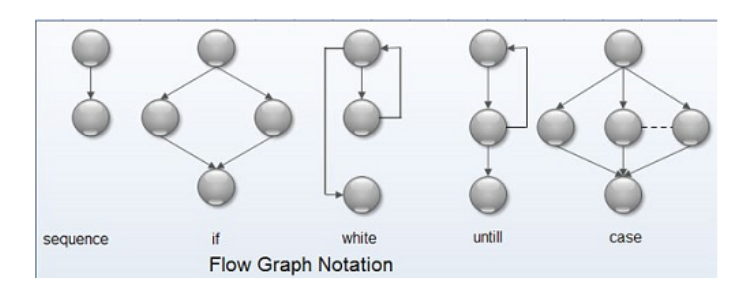
\includegraphics[scale=0.5]{pqr.png}
				\end{figure}
			
			\begin{figure}[h!]
					\centering
					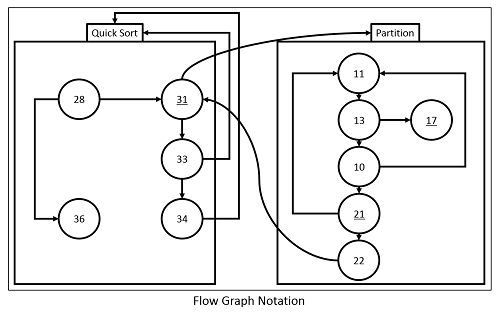
\includegraphics{hjv.png}
				\end{figure}	
			\noindent Sample Input: For integer array\\
			int A[] = $\{ 21,33,67,72,27,10,2,66,81,1\}$;
			Function is passed following arguments:\\
			$$quickSort(A, 0, 9);$$
			Output obtained:\\
			
			\noindent
			New partition: Low=0 High=9\\
			Swapped 21 with Pivot 1\\
			
			\noindent
			New partition: Low=1 High=9\\
			Swapped 33 with 10\\
			Swapped 67 with 2\\
			Swapped 72 with Pivot 21\\
			
			\noindent
			New partition: Low=1 High=2\\
			Swapped 10 with Pivot 2\\
			
			\noindent
			New partition: Low=4 High=9\\
			Swapped 27 with 27\\
			Swapped 33 with 33\\
			Swapped 67 with 67\\
			Swapped 66 with 66\\
			Swapped 81 with Pivot 72\\
			
			\noindent
			New partition: Low=4 High=7\\
			Swapped 27 with 27\\
			Swapped 33 with 33\\
			Swapped 67 with Pivot 66\\
			
			\noindent
			New partition: Low=4 High=5\\
			Swapped 27 with 27\\
			Swapped 33 with Pivot 33\\
			
			1,2,10,21,27,33,66,67,72,81,\\
			Note: \\
			The underlined nodes are the ones being tested.
			The above output shows that every test region is covered for given input.\\ 
			
			
			\subsection{ POSITIVE/NEGATIVE TESTING }
			
			\textbf{Positive Testing :}\\
			The element entered in ascending order then correct location of key will be found\\ 
			Example- Input  sequence(17)       key (17)         output(true ,1)\\ 
			
			\textbf{ Negative Testing :}\\
			The element  not entered in ascending order then wrong location of key will be found\\ 
			Example- Input  sequence(17)       key (0)         output(false,??)\\ 
			
			\subsection{ADVANCED TESTING TECHNIQUE}
			Google Testing Framework can be used in future for testing the code
			
\section{CONCLUSION : }
	We have studied divide and conquer strategies and have successfully implemented concurrent quick sort algorithm using c++ omp framework.

\end{document}